%%
%% This is file `sigconf.tex',
%% generated with the docstrip utility.
%%
%% The original source files were:
%%
%% samples.dtx  (with options: `all,proceedings,sigconf')
%% 
%% IMPORTANT NOTICE:
%% 
%% For the copyright see the source file.
%% 
%% Any modified versions of this file must be renamed
%% with new filenames distinct from sigconf.tex.
%% 
%% For distribution of the original source see the terms
%% for copying and modification in the file samples.dtx.
%% 
%% This generated file may be distributed as long as the
%% original source files, as listed above, are part of the
%% same distribution. (The sources need not necessarily be
%% in the same archive or directory.)
%%
%%
%% Commands for TeXCount
%TC:macro \cite [option:text,text]
%TC:macro \citep [option:text,text]
%TC:macro \citet [option:text,text]
%TC:envir table 0 1
%TC:envir table* 0 1
%TC:envir tabular [ignore] word
%TC:envir displaymath 0 word
%TC:envir math 0 word
%TC:envir comment 0 0
%%
%% The first command in your LaTeX source must be the \documentclass
%% command.
%%
%% For submission and review of your manuscript please change the
%% command to \documentclass[manuscript, screen, review]{acmart}.
%%
%% When submitting camera ready or to TAPS, please change the command
%% to \documentclass[sigconf]{acmart} or whichever template is required
%% for your publication.
%%
%%
\documentclass[sigconf]{acmart}
%%
%% \BibTeX command to typeset BibTeX logo in the docs
\AtBeginDocument{%
  \providecommand\BibTeX{{%
    Bib\TeX}}}

%% Rights management information.  This information is sent to you
%% when you complete the rights form.  These commands have SAMPLE
%% values in them; it is your responsibility as an author to replace
%% the commands and values with those provided to you when you
%% complete the rights form.
\setcopyright{acmlicensed}
\copyrightyear{2018}
\acmYear{2018}
\acmDOI{XXXXXXX.XXXXXXX}
%% These commands are for a PROCEEDINGS abstract or paper.
% \acmConference[Conference acronym 'XX]{Make sure to enter the correct
%   conference title from your rights confirmation email}{June 03--05,
%   2018}{Woodstock, NY}
%%
%%  Uncomment \acmBooktitle if the title of the proceedings is different
%%  from ``Proceedings of ...''!
%%
%%\acmBooktitle{Woodstock '18: ACM Symposium on Neural Gaze Detection,
%%  June 03--05, 2018, Woodstock, NY}
\acmISBN{978-1-4503-XXXX-X/2018/06}


%%
%% Submission ID.
%% Use this when submitting an article to a sponsored event. You'll
%% receive a unique submission ID from the organizers
%% of the event, and this ID should be used as the parameter to this command.
%%\acmSubmissionID{123-A56-BU3}

%%
%% For managing citations, it is recommended to use bibliography
%% files in BibTeX format.
%%
%% You can then either use BibTeX with the ACM-Reference-Format style,
%% or BibLaTeX with the acmnumeric or acmauthoryear sytles, that include
%% support for advanced citation of software artefact from the
%% biblatex-software package, also separately available on CTAN.
%%
%% Look at the sample-*-biblatex.tex files for templates showcasing
%% the biblatex styles.
%%
%%
%% The majority of ACM publications use numbered citations and
%% references.  The command \citestyle{authoryear} switches to the
%% "author year" style.
%%
%% If you are preparing content for an event
%% sponsored by ACM SIGGRAPH, you must use the "author year" style of
%% citations and references.
%% Uncommenting
%% the next command will enable that style.
%%\citestyle{acmauthoryear}
\usepackage{tikz}
\usepackage{graphicx}

%%
%% end of the preamble, start of the body of the document source.
\begin{document}

%%
%% The "title" command has an optional parameter,
%% allowing the author to define a "short title" to be used in page headers.
\title{Final Project Proposal}

%%
%% The "author" command and its associated commands are used to define
%% the authors and their affiliations.
%% Of note is the shared affiliation of the first two authors, and the
%% "authornote" and "authornotemark" commands
%% used to denote shared contribution to the research.

\author{Juntang Wang}
\affiliation{%
  \institution{Harvard University}
  \city{Cambridge}
  \country{USA}}
\email{juntangwang@g.harvard.edu}

\author{Ciro Zhang}
\affiliation{%
  \institution{Harvard University}
  \city{Cambridge}
  \country{USA}}
\email{cirozhang@g.harvard.edu}


%%
%% By default, the full list of authors will be used in the page
%% headers. Often, this list is too long, and will overlap
%% other information printed in the page headers. This command allows
%% the author to define a more concise list
%% of authors' names for this purpose.

%%
%% The abstract is a short summary of the work to be presented in the
%% article.


\begin{abstract}
TBA
\end{abstract}


% \received{20 February 2007}
% \received[revised]{12 March 2009}
% \received[accepted]{5 June 2009}

%%
%% This command processes the author and affiliation and title
%% information and builds the first part of the formatted document.
\maketitle
% Preamble: \usepackage{tikz,graphicx}
% AI-assisted schematic; the toy numbers are not experimental results.

\begin{figure*}[t]
\centering
\resizebox{0.85\textwidth}{!}{%
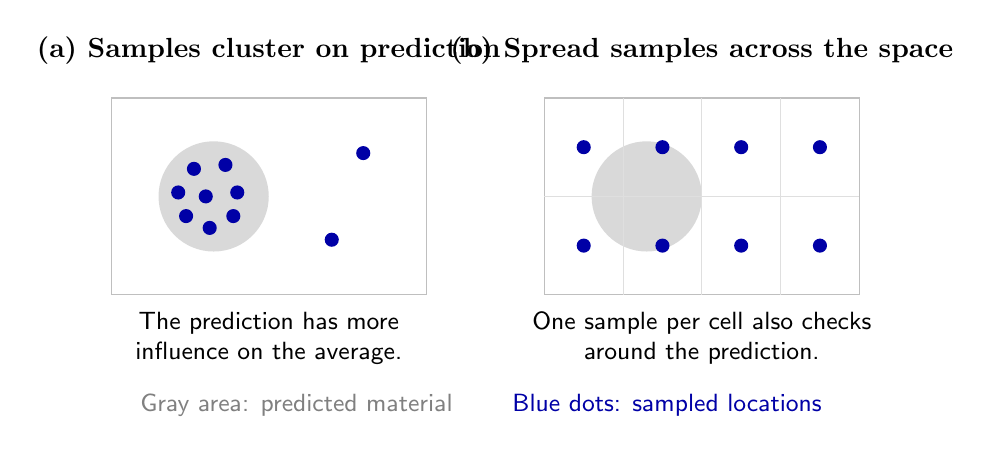
\begin{tikzpicture}[
    font=\sffamily\small,
    sample/.style={circle,fill=blue!65!black,
                   inner sep=1.8pt}
]

\begin{scope}
    \node[font=\bfseries] at (2,3.1)
        {(a) Samples cluster on prediction};

    \draw[gray!50] (0,0) rectangle (4,2.5);
    \fill[gray!30] (1.3,1.25) circle (0.7);

    \foreach \x/\y in {
        0.95/1.0, 1.25/0.85, 1.55/1.0,
        0.85/1.3, 1.2/1.25, 1.6/1.3,
        1.05/1.6, 1.45/1.65,
        2.8/0.7, 3.2/1.8
    }
        \node[sample] at (\x,\y) {};

    \node[align=center,text width=4.5cm] at (2,-0.55)
        {The prediction has more influence on the average.};
\end{scope}

\begin{scope}[xshift=5.5cm]
    \node[font=\bfseries] at (2,3.1)
        {(b) Spread samples across the space};

    \draw[gray!50] (0,0) rectangle (4,2.5);
    \fill[gray!30] (1.3,1.25) circle (0.7);

    \foreach \x in {1,2,3}
        \draw[gray!25] (\x,0)--(\x,2.5);
    \draw[gray!25] (0,1.25)--(4,1.25);

    \foreach \x in {0.5,1.5,2.5,3.5}
        \foreach \y in {0.625,1.875}
            \node[sample] at (\x,\y) {};

    \node[align=center,text width=4.5cm] at (2,-0.55)
        {One sample per cell also checks\\
         around the prediction.};
\end{scope}

\node[align=center] at (4.75,-1.4) {
    \textcolor{gray}{Gray area: predicted material}
    \qquad
    \textcolor{blue!65!black}{Blue dots: sampled locations}
};

\end{tikzpicture}%
}
\caption{Draft figure of our hypothesis: clustered samples may reinforce a false prediction.}
\label{fig:sampling-hypothesis}
\end{figure*}


\section{Research goal and problem statement}

Reconstructing a 3D scene from only a few images is challenging because different geometric configurations can reproduce the same observed views. Consequently, a Neural Radiance Field (NeRF) may fit its training images while still producing floating artifacts or incorrect geometry when task to rendered from new viewpoints. Thus, photometric reconstruction loss alone does not sufficiently constrain scene geometry, as an incorrect configuration can still reproduce the observed images. Improving reconstruction under limited observations is important for applications where capturing dense image collections is impractical.

DriftNeRF (cite here) addresses this problem by encouraging the model to predict similar densities at nearby points sampled along different camera rays. For each point, it computes a target density by averaging neighboring predictions, giving more weight to closer points. However, the candidate points are still drawn from the renderer's existing samples, whose spatial distribution depends on camera coverage and ray sampling. Thus, uniform selection from this pool does not necessary imply the uniform coverage of the underlying 3D neighborhood. Regions containing more samples can therefore contribute more strongly to the consensus target.

This raises an open research question: how much does density consensus reflect the actual reconstructed geometry, and how much does it depend on where samples are concentrated? We hypothesize that this dependence can sometimes reinforce incorrect density estimates. For example, concentrating samples around an incorrectly reconstructed density peak could increase that region's influence on nearby targets. However, surface-focused sampling may also provide useful guidance by emphasizing genuine structures. The effect of balancing these contributions must therefore be investigated empirically.

This project will study how sample placement affects density consensus and test an alternative that uses more evenly distributed points within each local neighborhood. The main challenges we foresee are separating sampling effects from changes in the learned geometry, preserving thin structures, and keeping the extra computation manageable. We will use a small subset of NeRF-Synthetic, focusing on static scenes with known camera poses and only a few input views. Our goal is to determine when balanced sampling makes consensus targets less sensitive to sample placement and whether this leads to better reconstruction from new viewpoints.


\section{Relationship to prior work}

Many existing works on sparse-view NeRF introduce additional constraints to reduce overfitting and improve novel-view synthesis. For example, FreeNeRF uses progressive frequency regularization to control the complexity of the learned field during training and penalizes density near cameras to reduce artifacts. Our previous work like DriftNeRF encourages nearby points sampled along different camera rays to have similar density predictions. 

This project directly builds on DriftNeRF but examines the sampling distribution underlying this consensus computation. Although the distance kernel determines the weight of each candidate, the spatial concentration of candidates can also affects the resulting average. Thus, we will investigate this interaction while retaining the original field representation and photometric objective.

The intended contribution is a controlled analysis of sampling dependence and an evaluation of spatially balanced consensus construction. We do not assume that uniform spatial coverage is always preferable so the experiments will examine the tradeoff between reducing disproportionate sample influence and retaining useful emphasis on scene surfaces.


\section{Proposed Method}

The following is a draft of the proposed method we will do for this project. 

\paragraph{Testing the effect of sampling.}
We will first take a trained NeRF and keep its predictions fixed. For the same set of anchor points, we will change how nearby points are sampled and compare the resulting density averages. We will use the same number of candidate points for each sampling method and repeat the experiment to check whether differences are consistent or caused by randomness.

\paragraph{Balanced neighborhood sampling.}
Our proposed change is to spread candidate points more evenly around each anchor. We will divide a small 3D neighborhood into equal-sized cells and sample one point from each cell. We will then use the NeRF to predict the density at each point and calculate a weighted average, giving closer points more weight. This average becomes the target density for the anchor. The method uses the existing model and does not require additional images or depth information.

\paragraph{Training.}
We will keep the original image reconstruction loss and add a penalty when an anchor's density differs from its neighborhood average. The average will be treated as a fixed target during each update using stop-gradient. We will keep the original warmup schedule so that the model can begin learning the scene before applying this penalty.

\paragraph{Evaluation.}
We will compare standard NeRF, original DriftNeRF, and our modified version using three training images per scene. We will measure image quality using PSNR, SSIM, and LPIPS, and inspect whether floating artifacts are reduced while thin structures remain visible. We will also compare training time and the number of density queries. Finally, we will compare our cell-based sampling with randomly placed local points and test a few neighborhood sizes, sample counts, and penalty strengths.

\section{Experimental results}



\section{Conclusion} 


\section{Contributions and AI usage acknowledgement}


\bibliographystyle{ACM-Reference-Format}
\bibliography{sample-base}





\end{document}
\endinput
%%
%% End of file `sigconf.tex'.
